\subsection{La visión por computadora como área de estudio}
\subsubsection{Definición de visión por computadora}

La visión por computadora es un campo de la inteligencia artificial que hace posible que las máquinas tengan la capacidad de replicar tareas cognitivas humanas fundamentales tales como procesar, describir, analizar e interpretar con el fin de extraer información desde entradas visuales, es decir, imágenes y videos. Para llevar a cabo estas tareas, hace uso del \textbf{aprendizaje automático o del aprendizaje profundo}, lo que a su vez permite realizar tareas más complejas y específicas propias del campo, basadas en las fundamentales \cite{microsoftazure_computervision}.

\subsubsection{Tareas de visión por computadora}
Según IBM \cite{ibm_computer_vision}, la visión por computadora incluye las siguientes tareas:
\begin{itemize}
    \item Reconocimiento de imágenes
    \item Clasificación de imágenes
    \item Detección de objetos
    \item Segmentación de imágenes
    \item Seguimiento de objetos
    \item Comprensión de la escena
    \item Reconocimiento facial
    \item Estimación de pose
    \item Reconocimiento óptico de caracteres
    \item Generación de imágenes
    \item Inspección visual
\end{itemize}

\begin{figure}[H]
    \centering
    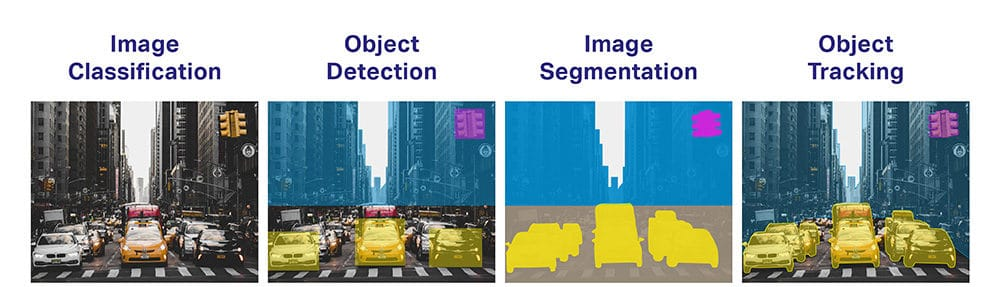
\includegraphics[width=1.0\textwidth]{images/C3/tareasVCOMP.jpg}
    \caption{Algunas tareas de visión por computadora}
    \label{fig:tareas_vc}
\end{figure}

Estas tareas representan, sin duda, la gran capacidad de la visión por computadora para poder resolver un amplio catálogo de problemas a partir del análisis de entradas visuales. No obstante, es importante tomar en cuenta el objetivo principal del problema de interés para delimitar el tipo o los tipos de tarea que se requieren abordar y, de esta manera, conseguir el tipo de información que se desea obtener.

\subsubsection{Herramientas y marcos de trabajo utilizadas en visión por computadora}

IBM \cite{ibm_computer_vision} señala que, para desarrollar ágilmente un sistema utilizando visión por computadora, es necesario el uso de diferentes herramientas y marcos de trabajo, entre los cuales se encuentran:

\begin{itemize}
    \item Keras
    \item OpenCV
    \item Scikit-image
    \item TensorFlow
    \item Torchvision
\end{itemize}

En cuanto al tratamiento de información, destacan las \textit{bibliotecas} \textbf{OpenCv y Scikit-image}, herramientas especializadas en el procesamiento digital de imágenes, detección de objetos, segmentación de imágenes y extracción de características, tareas que son realizadas mediante una gran colección de algoritmos de visión artificial \cite{ibm_computer_vision}.

En cambio, en lo que refiere al diseño, entrenamiento, despliegue y gestión de modelos de visión por computadora, \textbf{Keras} destaca siendo una \textit{interfaz de programación} orientada al aprendizaje profundo, la cual puede ejecutarse sobre los marcos de trabajo \textbf{TensorFlow} (que también constituye una de las plataformas de aprendizaje automático más extendidas) y \textbf{Pytorch}. Dentro de éste último se encuentran herramientas como \textbf{Torchvision}, que ofrece transformaciones de imágenes, conjuntos de datos y modelos preentrenados para clasificación, detección y segmentación \cite{ibm_computer_vision}.

\subsubsection{Flujo de trabajo común en el desarrollo de sistemas mediante visión por computadora}

Una vez definido y delimitado el problema a resolver, se requiere transformar la información visual en resultados útiles para la tarea o tareas específicas en que se plantea dicho problema, esto es, seguir un flujo de trabajo desde la adquisición de datos hasta la generación de una salida interpretable.

De acuerdo con IBM \cite{ibm_computer_vision}, es posible identificar una serie de etapas comunes que conforman el flujo de trabajo de un sistema de visión por computadora:

\begin{enumerate}
    \item Recopilación de datos
    \item Preprocesamiento
    \item Selección de modelos
    \item Entrenamiento del modelo
\end{enumerate}

Como se puede observar, este flujo suele comenzar con la \textbf{recopilación de imágenes} mediante cámaras o sensores, etapa en la cual se obtienen todos los datos visuales que servirán como entrada del sistema \cite{ibm_computer_vision}.

Después, en la etapa del \textbf{preprocesamiento}, estos datos visuales se someten a un tratamiento de limpieza en donde se mejora su calidad, por ejemplo, mediante el ajuste del brillo, el contraste, el tamaño, entre otras propiedades que ayuden a resaltar características relevantes para el análisis de los datos \cite{ibm_computer_vision}.

Una vez preparadas las imágenes, se realiza una comparativa entre los modelos candidatos a ser implementados en el sistema, tomando en cuenta que el \textbf{modelo que va a ser seleccionado} deberá ser el más conveniente con base en los objetivos del problema a resolver e ídoneo para cumplir con los objetivos de calidad. IBM señala que “seleccionar el modelo de machine learning adecuado es crucial para optimizar la eficiencia y el rendimiento” \cite{ibm_computer_vision}.

Por consiguiente, el \textbf{modelo seleccionado es entrenado} con los datos recopilados al inicio. En esta última etapa, se evalúan los objetivos de calidad (como la eficiencia y el rendimiento) de forma iterativa con el fin de encontrar los parámetros óptimos para satisfacer la tarea de visión artificial a la que está sujeto \cite{ibm_computer_vision}.

Finalmente, el sistema genera la salida deseada conforme a la tarea para la cual el modelo fue entrenado.

